\begin{appendices}
    \crefalias{section}{appsec}
    \section{Implementation} \label{app:Implementation}
    The code can be found here[]. \\
    Both the Identification and the Pricing Problem were programmed in Python 2.7 using NumPy 1.12.1, SciPy 0.19.1 and Pytorch 0.1.12 modules [web cites] \cite{SCPOptimizeDocs}\cite{NPDocs}. [Results from Python plotted in Matplotlib 2.0.2] With some code optimizations, the input dataset $\matr{F}$ was built using NumPy's \texttt{ndarray} and Pytorch's \texttt{tensor} functions. Since Pytorch offers NumPy-like code base but with dedicated neural network functions and submodules, Pytorch's \texttt{relu} and \texttt{softmax} functions were used along with other matrix operations.\\
    
    \subsection{Specific Implementation Details for the Pricing Problem}
    Among all the code optimizations in both models, some in that for the Pricing Problem are worth discussing, as they drastically differ from Algorithm \ref{alg:Solving the Pricing Problem} or are intricate. Most optimizations relevant to the Identification Problem are trivial and relate directly to those for the Pricing Problem. Therefore, only those in the Pricing Problem model are discussed.
    
    \subsubsection{Building the Dataset $\matr{F}$}
    Notice that we build the dataset $\matr{F}$ and batch-multiply it with $\matr{w_1}$ on each iteration/epoch (lines 2-3 of Algorithm \ref{alg:Solving the Pricing Problem}). Doing these steps are repetitive as most elements of $\matr{F}$, distances $\matr{D}$ and environmental feature vector $\vect{f}$, do not change unlike rewards $\vect{r}$. Moreover since $\matr{w_1}$ is fixed, Algorithm \ref{alg:Solving the Pricing Problem} would repetitively multiply the $\vect{f}$ and $\matr{D}$ components of $\matr{F}$ with $\matr{w_1}$. To avoid these unnecessary computations, we preprocessed most of $\matr{F}$ by batch-multiplying with $\matr{w_1}$ and only multiplied $\vect{r}$ with the corresponding elements of $\matr{w_1}$. Figure \ref{fig:Splitting and Batch Multiplying F and w1} describes the process graphically.\\
    \begin{figure}[!htbp]
        \centering
        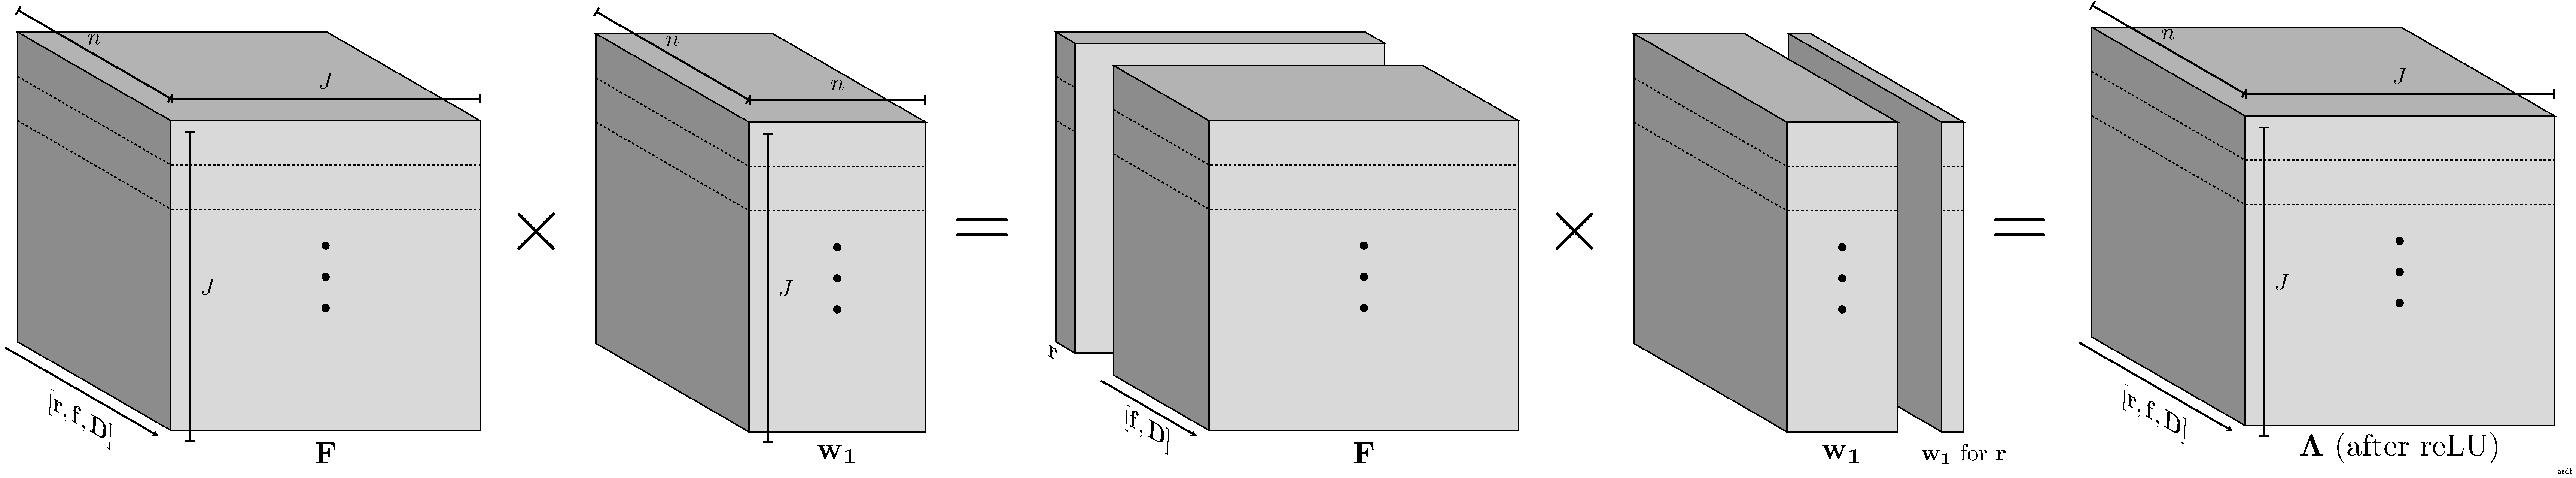
\includegraphics[width=\linewidth]{split_and_batch_multiply}
        \caption{Splitting and Batch Multiplying $\matr{F}$ and $\matr{w_1}$}
        \label{fig:Splitting and Batch Multiplying F and w1}
    \end{figure}    
    Although this preprocessing might seem applicable for the model in Identification Problem too, it does not apply fully. Since the weights $\matr{w_1}$ are updated on each iteration/epoch, we cannot multiply them with parts of $\matr{F}$ beforehand (Algorithm \ref{alg:Algorithm for the Identification Problem}). However, we can combine $\matr{D}$ and $\vect{f}$ in the preprocessing stage and simply append $\vect{r}[t]$ on each iteration, saving computation time.
    
    \subsubsection{Modeling the Linear Programming Problem in the Standard Format}
    The \texttt{scipy.optimize} module's \texttt{linprog} function requires that the arguments are in standard LP format. As discussed in \cref{sec:Calculating Rewards}, Equation \ref{eqn:lp_code_constrain_rewards} resembles the standard format more closely than \ref{eqn:lp_math_constrain_rewards}, but it may not be clear how so.\\
    
    Considering $\vect{u}$ and $\vect{r'}$ as variables $\vect{x}$, Equation \ref{eqn:lp_code_constrain_rewards} translates into Equation \ref{eqn:lp_matrix_rewards} ($J$ is the number of locations).
    \begin{equation} \label{eqn:lp_matrix_rewards}
    \begin{aligned}
    & \text{minimize}
    & & \begin{bmatrix}
    \vect{0_J}\\
    \vect{1_J}\\
    \end{bmatrix}^T
    \begin{bmatrix}
    \vect{r'}\\
    \vect{u}
    \end{bmatrix}\\ \\
    & \text{subject to}
    & & \begin{bmatrix}
    I_J & -I_J\\
    -I_J & -I_J\\
    \vect{1}^T_J & \vect{0}^T_J\\
    \end{bmatrix}
    \begin{bmatrix}
    \vect{r'}\\
    \vect{u}\\
    \end{bmatrix} \leq
    \begin{bmatrix}
    \vect{r}\\
    -\vect{r}\\
    \mathcal{R}\\
    \end{bmatrix}\\
    &&& r'_i, u_i \geq 0
    \end{aligned}
    \end{equation}
    
    \section{Strange GPU Speedup in LP Computation} \label{app:Strange GPU Speedup in LP Computation}
    Even though we intentionally transferred the rewards vector to and constrained it using \texttt{scipy.optimize} module's \texttt{linprog} function on the CPU, we obtained an unexpected GPU speedup in the LP runtimes (see \cref{sec:PriProbRes - GPU} and Figure \ref{fig:Finding Rewards - Time taken by the LP}). Confounded by this weird behavior, we wanted to pinpoint the reason(s) because SciPy's function could not have differentiated between the configurations and delivered different results. However, since this was not our research's prime motive, we did not take a strong quantitative approach in determining the cause(s).
    
    \subsection{Possible Reasons for GPU Speedup} \label{app:Possible Reasons for GPU Speedup}
    There could have been many reasons for this bizarre behavior, including but not limited to:
    \begin{enumerate}
        \item SciPy's Optimize Module differentiating between configurations. This can be ruled out because the module could not have known the configuration during which it was called. This is because the configuration settings were applicable only on user-programmed operations, and needed to be explicitly stated - as mandated by Pytorch \cite{PTDocs}. SciPy's Optimize Module identifying the configurations is just supernatural.
        \item CPU ``set'' using exploiting more main memory than GPU ``set''. We suspected that since CPU ``set'' configuration's operations were executed solely on the CPU, the residing datasets could have used more main memory than when GPU ``set'' was running. This could have hampered the performance of LP with CPU ``set'', as the LP had lesser space to operate in. Unlike the 1\textsuperscript{st} possibility, this would have meant that CPU ``set'' was slowing down the LP, and not that GPU ``set'' was speeding up the LP.
        \item Neural network in CPU ``set'' using more CPU threads than that in GPU ``set''. The Intel i7-7700K processor is quad-core with 8 threads. Since Pytorch uses OpenMP \cite{PTDocs}, a parallel processing API for CPUs, we fancied the neural network to utilize more threads than that in GPU ``set'', thus allowing less available threads for the LP to run. 
        
        However, given that our scripts in Python did not explicitly use parallel programming with CPU ``set'' and the code was sequential, one could very well suggest that upon completion of the neural network, all threads should have been synchronized, after which the LP would have started. This would have meant that the LP's resources would have been independent of the neural network's resources, raising questions on this possibility.
    \end{enumerate}

    \subsection{LP Slowing Down or Speeding Up?} \label{app:LP Slowing Down or Speeding Up?}
    First we determined whether the LP runtime was being sped up with GPU ``set'' or slowed down with CPU ``set''. To test this, we created a copy of our Pricing Problem's model, which focused only on logging LP runtimes at each epoch. For a baseline comparison, we scripted the same LP \textit{without} the neural network, which gave us the \underline{original} runtimes for the LP (ran for equal number of epochs), without any involvement of Pytorch modules or functions. 
    
    Comparing the former runtimes (CPU and GPU ``set'') with `Only LP' runtime (independent script) in Figure \ref{fig:LP Runtime Example for Different Configurations}, we observed that the LP in the CPU ``set'' configuration took longer to execute than that in  `Only LP' setting during each epoch. We also noticed little to no interaction between the neural network in GPU ``set'' with the LP, as the runtimes of LP in GPU ``set'' were similar to those of LP in `Only LP' setting. This confirmed that CPU ``set'' was slowing down the LP and GPU ``set'' was not speeding it up. But why?
    \begin{figure}[!htbp]
        \centering
        \begin{tikzpicture}
        \begin{axis}[
            width=\textwidth,
            height=8cm,
            xlabel=Epochs,
            ylabel=Time/s,
            scaled y ticks = false,
            grid=both,
            every axis plot/.append style={very thick},
        ]
        \addplot[red] table [col sep=comma,x=epoch, y=cpuset]{datafiles/lp_time_logs.csv};
        \addlegendentry{CPU ``set''}
        
        \addplot[blue] table [col sep=comma,x=epoch, y=gpuset]{datafiles/lp_time_logs.csv};
        \addlegendentry{GPU ``set''}
        
        \addplot[brown] table [col sep=comma,x=epoch, y=onlylp]{datafiles/lp_time_logs.csv};
        \addlegendentry{`Only LP'}
        
        \end{axis}
        \end{tikzpicture}
        \caption[LP Runtime Example for Different Configurations]{LP Runtime Example for Different Configurations: LPs in both CPU and GPU ``set'' start running slowly, but pick up speed after $\approx$ 20 epochs. We could not explain the presence of spikes in LP runtimes of CPU ``set'' and their absence in GPU ``set''. The test was done on a random dataset for 200 epochs, while the other experiment specifications were same as in \cref{sec:Experiment Specifications}.}
        \label{fig:LP Runtime Example for Different Configurations}
    \end{figure}
    
    \subsection{CPU and Main Memory Usage} \label{app:CPU and Main Memory Usage}
    While logging the LP runtimes in \cref{sec:LP Slowing Down or Speeding Up?}, we also recorded an estimate of the amount of computer resources both configurations were using. Using the \texttt{top} package in Ubuntu, we polled the resource monitor every 0.1 seconds while the python script was running\footnote{\label{foo:logs not epochs} Running processes were polled every 0.1 seconds - contributing to a `log'. The longer the script ran, the more logs collected.}. Figures \ref{fig:CPU Usage by Different Configurations} and \ref{fig:Main Memory Usage by Different Configurations} shows how much main memory and CPU resource each setting was using.
    
    It is fascinating to see that CPU ``set'' constantly used more than 4 out of 8 available threads, i.e., $>400 \%$ CPU usage, during execution, while GPU ``set'' only used a single thread. Also, since we polled at every 0.1 second, and the LP took a minimum of 0.14 seconds (Figure \ref{fig:LP Runtime Example for Different Configurations}), the data displayed in Figure \ref{fig:CPU Usage by Different Configurations} must show resource use \textit{while} the LP was running. Considering that the LP in `Only LP' setting only used a single thread (100 \%), it makes sense that GPU ``set'' would use 1 thread for execution - the neural network operations were performed on the GPU, leaving the CPU empty for management and LP. On the other hand, it is apparent that CPU ``set'' had multi-threaded operations running simultaneously, even though we reasoned its low possibility (\#3 in \cref{sec:Possible Reasons for GPU Speedup}). Since we know from the `Only LP' setting that the LP only used a single thread, the other threads in CPU ``set'' must have been the neural network. Although this counters our reasoning that the neural network threads should have synchronized before the LP started, it seems that those threads were still active. While we cannot explain this behavior, this activity does not impact correctness, as found from optimization tests on CPU ``set''\footnote{CPU ``set'' tests were done for optimization on original datasets to check this. Since we got the same results as for GPU ``set'' optimization tests \cref{sec:PriProbRes - Optimization}, the results are not shown in the report.} (same optimization figures as obtained for GPU ``set'' - \cref{sec:PriProbRes - Optimization}).
    
    On the other hand, GPU ``set'' was using 10 times as much main memory as CPU ``set'' or `Only LP', even though all matrix operations were executed and stored on the GPU. Not only this is weird, but it is also opposite of what we expected to happen - CPU ``set'' using more main memory and hampering LP performance. It is ironic that the LP performs better (even as good as `Only LP') on GPU ``set'' even when the configuration uses a lot more main memory than CPU ``set''. Clearly, the main memory usage cannot be a criterion for assessing LP performance on different configurations.
    \begin{figure}[!htbp]
        \centering
        \begin{minipage}{.49\textwidth}
            \centering
            \begin{tikzpicture}
            \begin{axis}[
            name=cpuusage-cpuset,
            width=\textwidth,
            enlarge x limits=0.15,
            no markers,
            ymax=800,
            ymin=0,
            ]
            \addplot+[fill=red, opacity=.4] table [col sep=comma,x=epoch, y=cpu]{datafiles/ext_cpu_cpuset.csv} \closedcycle;
            
            \addplot+[very thick, red!50!black] table [col sep=comma,x=epoch, y=cpu]{datafiles/ext_cpu_cpuset.csv};
            
            \end{axis}
            
            \begin{axis}[
            name=cpuusage-gpuset,
            at=(cpuusage-cpuset.below south west), anchor=above north west,
            width=\textwidth,
            enlarge x limits=0.15,
            no markers,
            ylabel={CPU Usage/\%},
            ymax=200,
            ymin=0,
            ]
            \addplot+[fill=blue, opacity=.4] table [col sep=comma,x=epoch, y=cpu]{datafiles/ext_cpu_gpuset.csv} \closedcycle;
            
            \addplot+[very thick, blue!50!black] table [col sep=comma,x=epoch, y=cpu]{datafiles/ext_cpu_gpuset.csv};
            \end{axis}
            
            \begin{axis}[
            name=cpuusage-onlylp,
            at=(cpuusage-gpuset.below south west), anchor=above north west,
            width=\textwidth,
            enlarge x limits=0.15,
            no markers,
            xlabel={Logs},
            ymax=200,
            ymin=0,
            ]
            \addplot+[fill=green, opacity=.4] table [col sep=comma,x=epoch, y=cpu]{datafiles/ext_onlylp.csv} \closedcycle;
            
            \addplot+[very thick, green!50!black] table [col sep=comma,x=epoch, y=cpu]{datafiles/ext_onlylp.csv};
            \end{axis}
            \end{tikzpicture}
            \caption[CPU Usage by Different Configurations]{CPU Usage by Different Configurations\textsuperscript{\ref{foo:logs not epochs}}: From top - CPU ``set'', GPU ``set'', `Only LP'. CPU Usage for GPU ``set'' and `Only LP' are very similar as operations other than the LP run on the GPU.}
            \label{fig:CPU Usage by Different Configurations}
        \end{minipage}\hfill
        \begin{minipage}{.49\textwidth}
            \centering
            \begin{tikzpicture}
            \begin{axis}[
            name=memusage-cpuset,
            width=\textwidth,
            enlarge x limits=0.15,
            no markers,
            ymax=1,
            ymin=0,
            ]
            \addplot+[fill=red, opacity=.4] table [col sep=comma,x=epoch, y=mem]{datafiles/ext_cpu_cpuset.csv} \closedcycle;
            
            \addplot+[very thick, red!50!black] table [col sep=comma,x=epoch, y=mem]{datafiles/ext_cpu_cpuset.csv};
            
            \end{axis}
            
            \begin{axis}[
            name=memusage-gpuset,
            at=(memusage-cpuset.below south west), anchor=above north west,
            width=\textwidth,
            enlarge x limits=0.15,
            no markers,
            ylabel={Main Memory Usage/\%},
            ymax=10,
            ymin=0,
            ]
            \addplot+[fill=blue, opacity=.4] table [col sep=comma,x=epoch, y=mem]{datafiles/ext_cpu_gpuset.csv} \closedcycle;
            
            \addplot+[very thick, blue!50!black] table [col sep=comma,x=epoch, y=mem]{datafiles/ext_cpu_gpuset.csv};
            \end{axis}
            
            \begin{axis}[
            name=memusage-onlylp,
            at=(memusage-gpuset.below south west), anchor=above north west,
            width=\textwidth,
            enlarge x limits=0.15,
            no markers,
            xlabel={Logs},
            ymax=1,
            ymin=0,
            ]
            \addplot+[fill=green, opacity=.4] table [col sep=comma,x=epoch, y=mem]{datafiles/ext_onlylp.csv} \closedcycle;
            
            \addplot+[very thick, green!50!black] table [col sep=comma,x=epoch, y=mem]{datafiles/ext_onlylp.csv};
            \end{axis}
            \end{tikzpicture}
            \caption[Main Memory Usage by Different Configurations]{Main Memory Usage by Different Configurations\textsuperscript{\ref{foo:logs not epochs}}: From top - CPU ``set'', GPU ``set'', `Only LP'. The neural network doesn't occupy much main memory in CPU ``set'' - could be due to Python/Pytorch's garbage collection.}
            \label{fig:Main Memory Usage by Different Configurations}
        \end{minipage}
    \end{figure}

    \subsubsection{Inexplicable Behavior} \label{app:Inexplicable Behavior}
    The machine's resource logs while model execution defy our expectations starkly. Elaborated in \cref{sec:CPU and Main Memory Usage}, it is clear that Main Memory Usage does not explain the strange GPU Speedup in LP runtimes for CPU and GPU ``set''; instead, main memory logs show the opposite picture - with GPU ``set'' using $\approx$ 10 times as much main memory as CPU ``set'' or `Only LP'.
    
    On the other hand, CPU Usage logs do correspond with our LP runtime observations, but the former phenomenon is inexplicable, at least from our side. We believe that the neural network should stop executing and the threads should synchronize, before the LP starts. The LP on CPU ``set'' should then use just 1 thread, as with `Only LP' setting, forming high spikes in the CPU usage graph (top, Figure \ref{fig:CPU Usage by Different Configurations}). At odds with what we expect, the CPU Usage graph shows constant use of 4-5 threads with tiny spikes, which are natural, indicating that the neural network's threads were running \textit{along with} the LP. While this would have targeted the model's correctness on CPU ``set'' config., the results we obtained are same as those with GPU ``set''.
    
    Therefore, while CPU usage logs for the configurations might explain the strange GPU Speedup, CPU usage for CPU ``set'' is itself strange and inexplicable. Additionally, main memory usage in GPU ``set'' is inexplicably high. Although both these behaviors could be caused by Pytorch's implementation specifics, we cannot ensure this possibility. Further research and suggestions are welcome.
\end{appendices}